\subsubsection{Successful forecasts}
\textbf{Brazil Spring (June 2013)}
EMBERS, while missing the initial uptick, captured the increase in the order of
magnitude of the protest events during the Brazilian Spring and also captured
the spatial spread in the events, in addition to forecasting that this would be
a "General Population" protest.
\begin{figure}[H]
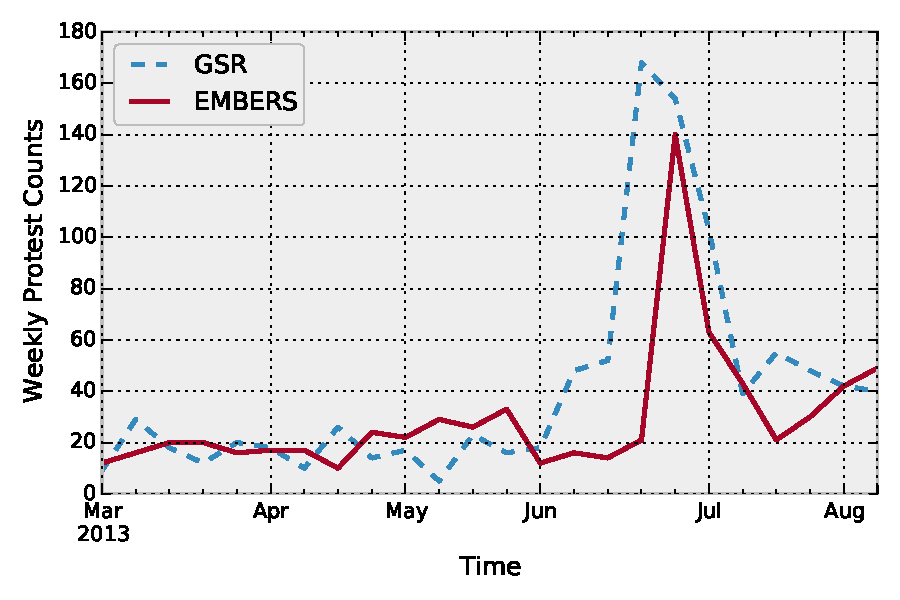
\includegraphics[width=.8\columnwidth]{cu/brazilJune13}
\caption{Brazil Spring}
\label{fig:brazilJune13}
\end{figure}


\textbf{Venezuelan Spring (Feb-March 2014)}
EMBERS captured some of the first `calls to protest` for the trigger city of
San Cristobal and its nearby surrounding areas and correctly forecast the
population (Education) and that the protests would turn violent. Over the next
days, EMBERS closely forecast the spike in the number of events and the spread
of the protests to additional cities.
   
\begin{figure}[H]
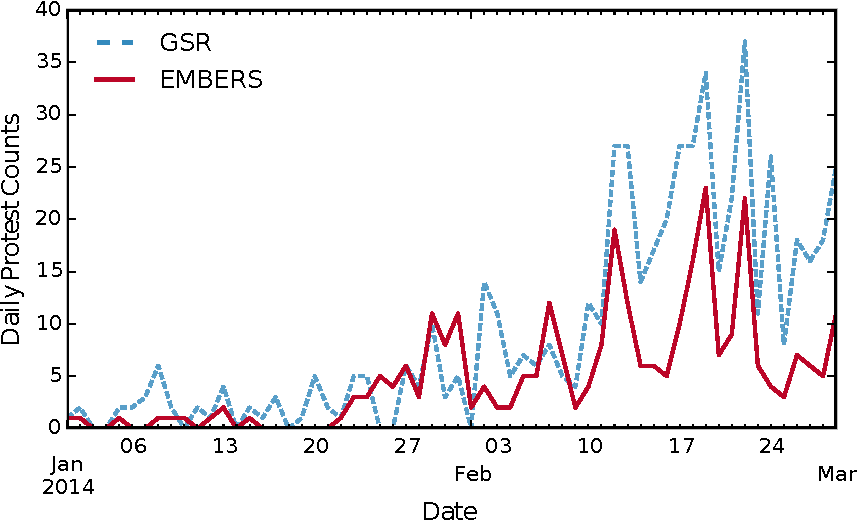
\includegraphics[width=.8\columnwidth]{cu/venezuelaFeb14}
\caption{Brazil Spring}
\label{fig:venezuelaMarch14}
\end{figure}

\textbf{Mexico Protests (October 2014)}[H]
EMBERS forecast an uptick of Mexico protests during early October 2014 stemming
from kidnappings and killings of student teachers, with a lead time of about 3
days. It also generated  a series of alert spikes coinciding with the first
large-scale nationwide protests between October 5th to 8th.
\begin{figure}
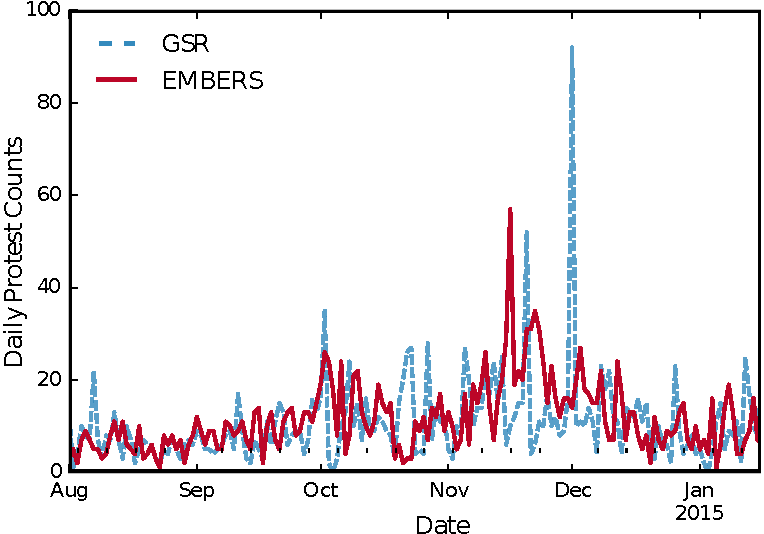
\includegraphics[width=.8\columnwidth]{cu/mexicoOct14}
\caption{Brazil Spring}
\label{fig:mexicoOct14}
\end{figure}

\textbf{Colombia (December'14 -March'15)}[H]

EMBERS successfully forecast the uptick in the number of events during the
middle of December 2014 and also the increase in protest counts during February
2015, though in the latter case EMBERS over predicted the counts. The uptick in
December 2014 was led by the opposition leader Alvaro Uribe against impunity.
Whereas the increase in  protest counts in February 2015
was due to trucker’s strike against increase in fuel price.

\begin{figure}
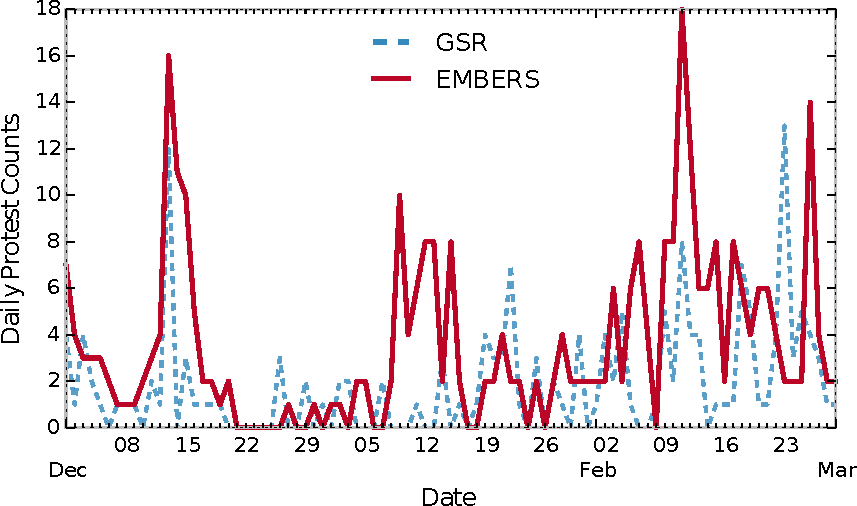
\includegraphics[width=.8\columnwidth]{cu/colombiaDec15}
\caption{Colombia Protests}
\label{fig:colombiaDec14}
\end{figure}

\textbf{Paraguay (February 2015)}[H]

EMBERS forecast the uptick in number of protest events in Paraguay during mid
February 2015. The events were mainly due to the lack of opportunity and basic
needs and against the introduction of new public-private partnership law.


\begin{figure}
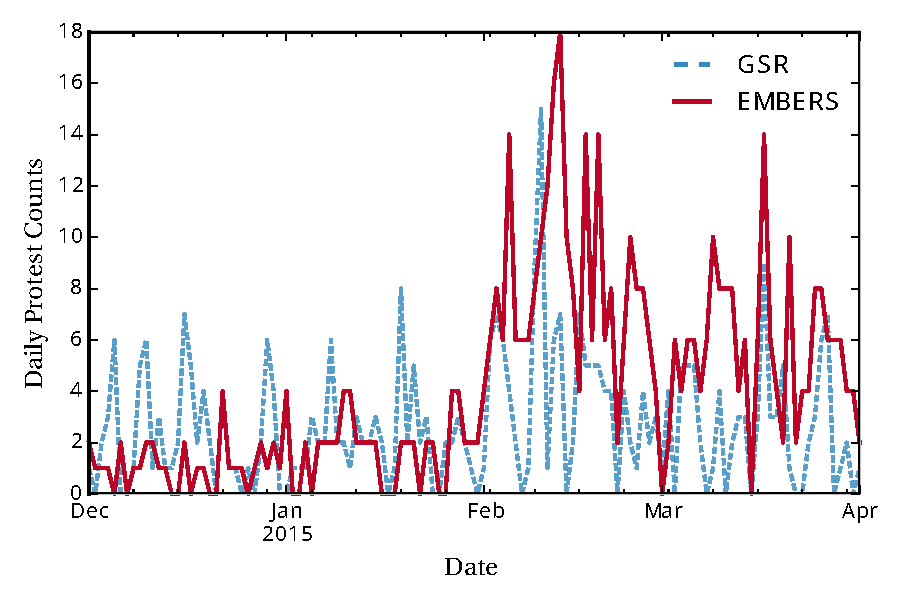
\includegraphics[width=.8\columnwidth]{cu/paraguayFeb15}
\caption{Paraguay Protests}
\label{fig:paraguay15}
\end{figure}

\textbf{Venezuelan Spring (Feb-March 2014)}[H]
EMBERS captured some of the first `calls to protest` for the trigger city of
San Cristobal and its nearby surrounding areas and correctly forecast the
population (Education) and that the protests would turn violent. Over the next
days, EMBERS closely forecast the spike in the number of events and the spread
of the protests to additional cities.

\begin{figure}
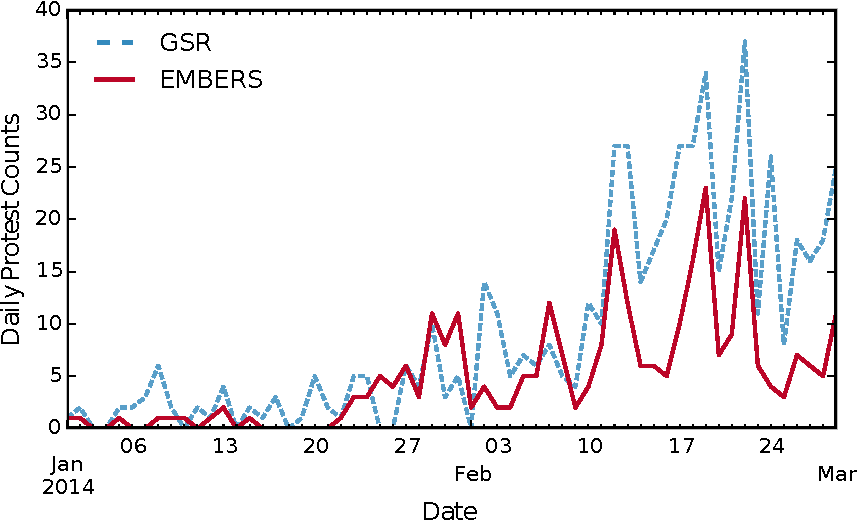
\includegraphics[width=.8\columnwidth]{cu/venezuelaFeb14}
\caption{Brazil Spring}
\label{fig:brazilSpring}
\end{figure}

\subsubsection{Failures}

some examples here
